%%%%%%%%%%%%%%%%%%%%%%%%%%%%%%%%%%%%%%%%%
% Jacobs Landscape Poster
% LaTeX Template
% Version 1.0 (29/03/13)
%
% Created by:
% Computational Physics and Biophysics Group, Jacobs University
% https://teamwork.jacobs-university.de:8443/confluence/display/CoPandBiG/LaTeX+Poster
% 
% Further modified by:
% Nathaniel Johnston (nathaniel@njohnston.ca)
%
% This template has been downloaded from:
% http://www.LaTeXTemplates.com
%
% License:
% CC BY-NC-SA 3.0 (http://creativecommons.org/licenses/by-nc-sa/3.0/)
%
%%%%%%%%%%%%%%%%%%%%%%%%%%%%%%%%%%%%%%%%%

%----------------------------------------------------------------------------------------
%	PACKAGES AND OTHER DOCUMENT CONFIGURATIONS
%----------------------------------------------------------------------------------------

\documentclass[final]{beamer}

\usepackage[scale=1.24]{beamerposter} % Use the beamerposter package for laying out the poster

\usepackage{wrapfig}

\usetheme{confposter} % Use the confposter theme supplied with this template

\setbeamercolor{block title}{fg=ngreen,bg=white} % Colors of the block titles
\setbeamercolor{block body}{fg=black,bg=white} % Colors of the body of blocks
\setbeamercolor{block alerted title}{fg=white,bg=dblue!70} % Colors of the highlighted block titles
\setbeamercolor{block alerted body}{fg=black,bg=dblue!10} % Colors of the body of highlighted blocks
% Many more colors are available for use in beamerthemeconfposter.sty

%-----------------------------------------------------------
% Define the column widths and overall poster size
% To set effective sepwid, onecolwid and twocolwid values, first choose how many columns you want and how much separation you want between columns
% In this template, the separation width chosen is 0.024 of the paper width and a 4-column layout
% onecolwid should therefore be (1-(# of columns+1)*sepwid)/# of columns e.g. (1-(4+1)*0.024)/4 = 0.22
% Set twocolwid to be (2*onecolwid)+sepwid = 0.464
% Set threecolwid to be (3*onecolwid)+2*sepwid = 0.708

\newlength{\sepwid}
\newlength{\onecolwid}
\newlength{\twocolwid}
\newlength{\threecolwid}
\setlength{\paperwidth}{48in} % A0 width: 46.8in
\setlength{\paperheight}{36in} % A0 height: 33.1in
\setlength{\sepwid}{0.024\paperwidth} % Separation width (white space) between columns
\setlength{\onecolwid}{0.22\paperwidth} % Width of one column
\setlength{\twocolwid}{0.464\paperwidth} % Width of two columns
\setlength{\threecolwid}{0.708\paperwidth} % Width of three columns
\setlength{\topmargin}{-0.5in} % Reduce the top margin size
%-----------------------------------------------------------

\usepackage{graphicx}  % Required for including images

\usepackage{booktabs} % Top and bottom rules for tables

%----------------------------------------------------------------------------------------
%	TITLE SECTION 
%----------------------------------------------------------------------------------------

\title{The Scintillator-Layered Imaging Microscope for Environmental Research} % Poster title

\author{\texorpdfstring{G. Buchanan$^1$, M. F. Kidd$^1$, S. R. Elliott$^2$, K. Rielage$^2$, J. N. Murdock$^1$, R. S. Pirkle$^1$}{}}% Author(s)

\institute{$^1$Tennessee Tech University, $^2$Los Alamos National Laboratory} % Institution(s)

%----------------------------------------------------------------------------------------

\begin{document}

\addtobeamertemplate{block end}{}{\vspace*{2ex}} % White space under blocks
\addtobeamertemplate{block alerted end}{}{\vspace*{2ex}} % White space under highlighted (alert) blocks

\setlength{\belowcaptionskip}{2ex} % White space under figures
\setlength\belowdisplayshortskip{2ex} % White space under equations

\begin{frame}[t] % The whole poster is enclosed in one beamer frame

\begin{columns}[t] % The whole poster consists of three major columns, the second of which is split into two columns twice - the [t] option aligns each column's content to the top

\begin{column}{\sepwid}\end{column} % Empty spacer column

\begin{column}{\onecolwid} % The first column

%----------------------------------------------------------------------------------------
%	OBJECTIVES
%----------------------------------------------------------------------------------------

\begin{alertblock}{Objectives}

\begin{itemize}
\item Pinpoint, with high position resolution, radioactive decay events with a wide range of energies.
\item Develop a Monte Carlo simulation to accurately model the experiment.
\item Ultimately, apply the results from SLIMER in environmental research fields, particularly with algae blooms--both preventing their formation, and developing their uses in mitigating atmospheric carbon dioxide.
\end{itemize}

\end{alertblock}

%----------------------------------------------------------------------------------------
%	INTRODUCTION
%----------------------------------------------------------------------------------------

\begin{block}{Introduction}

SLIMER's main potential is in the field of microbial ecology: identifying the microbes that process different nutrients within ecosystems in order to gain an understanding of those ecosystems. To this end, SLIMER incorporates a microcolumnar scintillator in a standard fluorescence microscope coupled with an EMCCD camera.

\hspace{1cm}

\begin{figure}
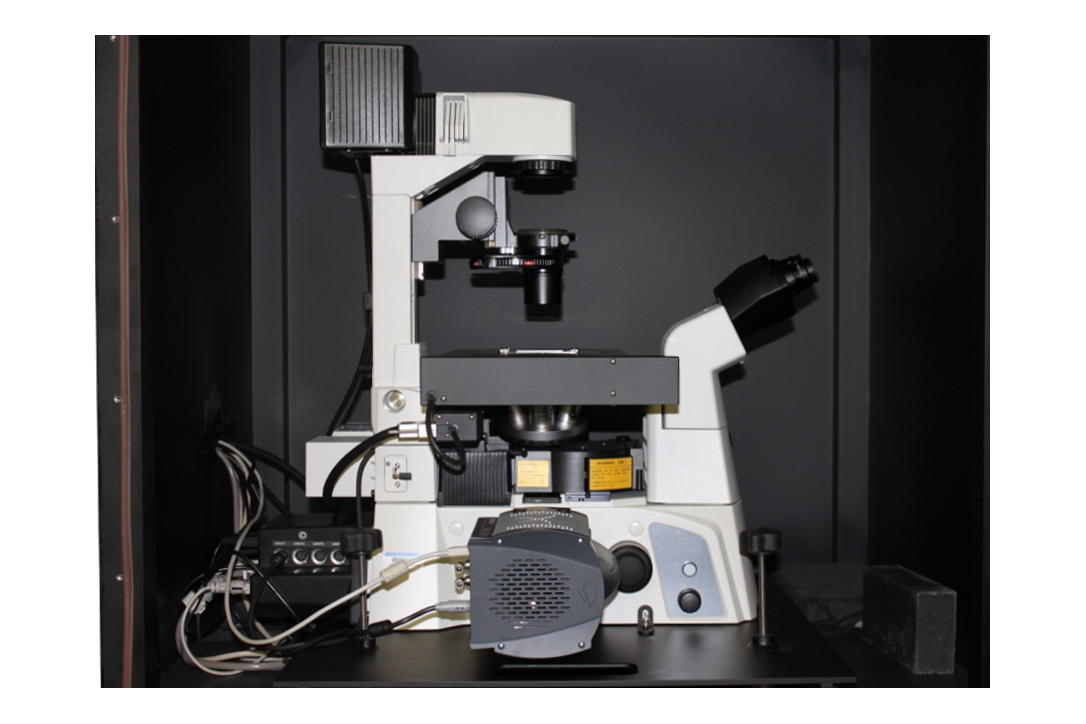
\includegraphics[width=\linewidth]{detector2.png}
\caption{Microscope and camera inside dark box.}
\end{figure}

A radioactive event interacts with the cesium iodide to create photons, which the camera detects. Events are displayed on a computer screen (see Figure \ref{fig:events}). 

\end{block}

\begin{center}
\begin{tabular}{ccc}

\includegraphics[width=0.3\linewidth]{TTU.png} & \hspace{3cm} & 
\includegraphics[width=0.3\linewidth]{lanl.png}
\end{tabular}
\end{center}

%----------------------------------------------------------------------------------------

\end{column} % End of the first column

\begin{column}{\sepwid}\end{column} % Empty spacer column

\begin{column}{\twocolwid} % Begin a column which is two columns wide (column 2)

\begin{columns}[t,totalwidth=\twocolwid] % Split up the two columns wide column

\begin{column}{\onecolwid}\vspace{-.6in} % The first column within column 2 (column 2.1)

%----------------------------------------------------------------------------------------
%	MATERIALS
%----------------------------------------------------------------------------------------

\begin{block}{Materials}

\begin{wrapfigure}{l}{0.5\textwidth}
	\centering
	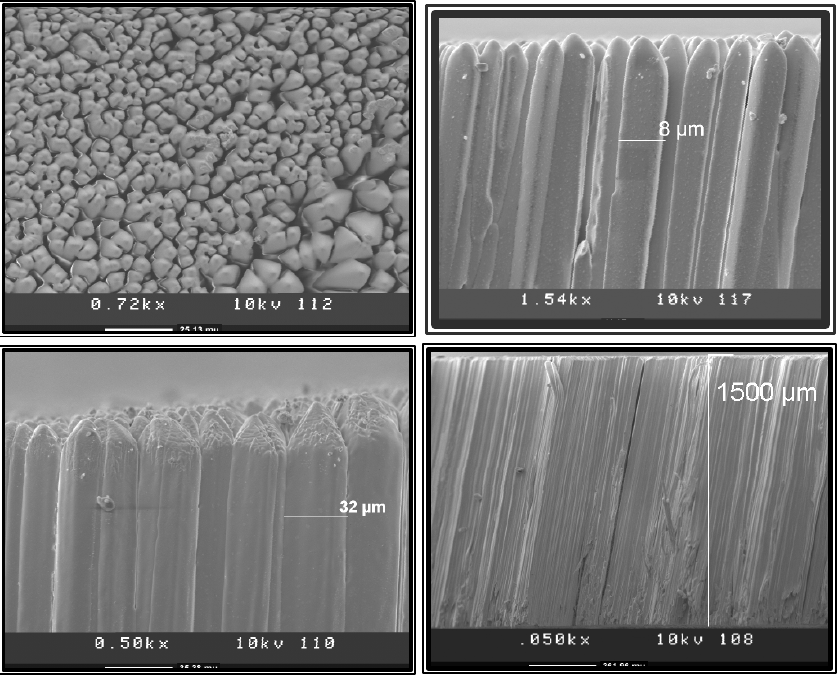
\includegraphics[width=0.8\linewidth]{csi.png}
    \caption{Microcolumnar \\CsI structure. Photo from [2].}
    \vspace{-40pt}
    \label{fig:csi_struct}
\end{wrapfigure}

A new EMCCD camera and new objectives were purchased, in order to reduce background noise and improve light collection efficiency. The camera and microscope are set up in a dark box. The camera software are Micro-Manager and ImageJ, an open source camera manager and image analyzer, respectively. The simulation, as well as various macros for image analysis, are written in C++ with \textsc{Geant}4 and ROOT.

\end{block}

%----------------------------------------------------------------------------------------

\end{column} % End of column 2.1

\begin{column}{\onecolwid}\vspace{-.6in} % The second column within column 2 (column 2.2)

%----------------------------------------------------------------------------------------
%	EXPERIMENT
%----------------------------------------------------------------------------------------

\begin{block}{Experiment}

\begin{figure}
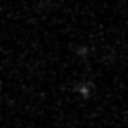
\includegraphics[width=0.35\linewidth]{c14.png}
\hspace{0.05\linewidth}
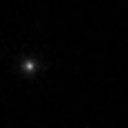
\includegraphics[width=0.35\linewidth]{am.jpg}
\caption{Left: $^{14}$C beta event. Right: $^{241}$Am alpha event.}
\label{fig:events}
\end{figure}

Events in the CsI show up in grayscale on the computer screen. Bright, distinct events, such as $^{241}$Am alpha particles, are much easier to detect than lower-energy, less distinct events, such as betas from $^{14}$C. 

\end{block}

%----------------------------------------------------------------------------------------

\end{column} % End of column 2.2

\end{columns} % End of the split of column 2 - any content after this will now take up 2 columns width

%----------------------------------------------------------------------------------------
%	FUTURE WORK
%----------------------------------------------------------------------------------------

\begin{alertblock}{Future Work}

Being able to determine the position of events is highly important. In the near future, work will go towards determining the spatial resolution for various sources. 

\end{alertblock} 

%----------------------------------------------------------------------------------------

\begin{columns}[t,totalwidth=\twocolwid] % Split up the two columns wide column again

\begin{column}{\onecolwid} % The first column within column 2 (column 2.1)

%----------------------------------------------------------------------------------------
%	SIMULATION
%----------------------------------------------------------------------------------------

\begin{block}{Simulation}

Simulations are used to find problems with the experiment, and to try different things before changing the physical setup. Data from the simulation can be compared to data collected from the experiment (see Figure \ref{fig:cs}) and, if needed, changes can be made to the experiment or the simulation.

\hspace{1cm}
\begin{figure}
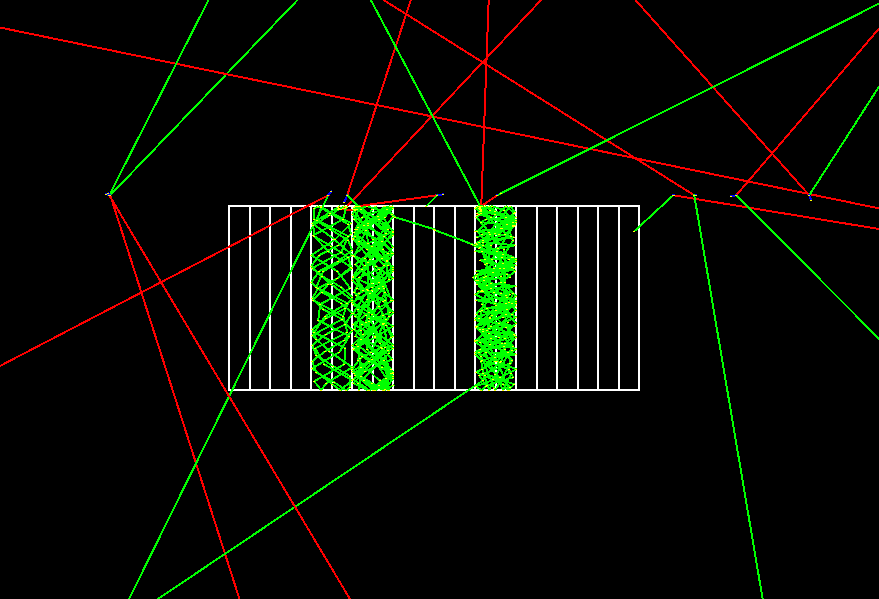
\includegraphics[width=0.8\linewidth]{events.png}
\caption{Initial radioactive decay events occurring outside the CsI. Three electrons interact with the CsI to generate photons.}
\end{figure}

\end{block}

%----------------------------------------------------------------------------------------

\end{column} % End of column 2.1

\begin{column}{\onecolwid} % The second column within column 2 (column 2.2)

%----------------------------------------------------------------------------------------
%	RESULTS
%----------------------------------------------------------------------------------------

\begin{block}{Results}

\begin{figure}
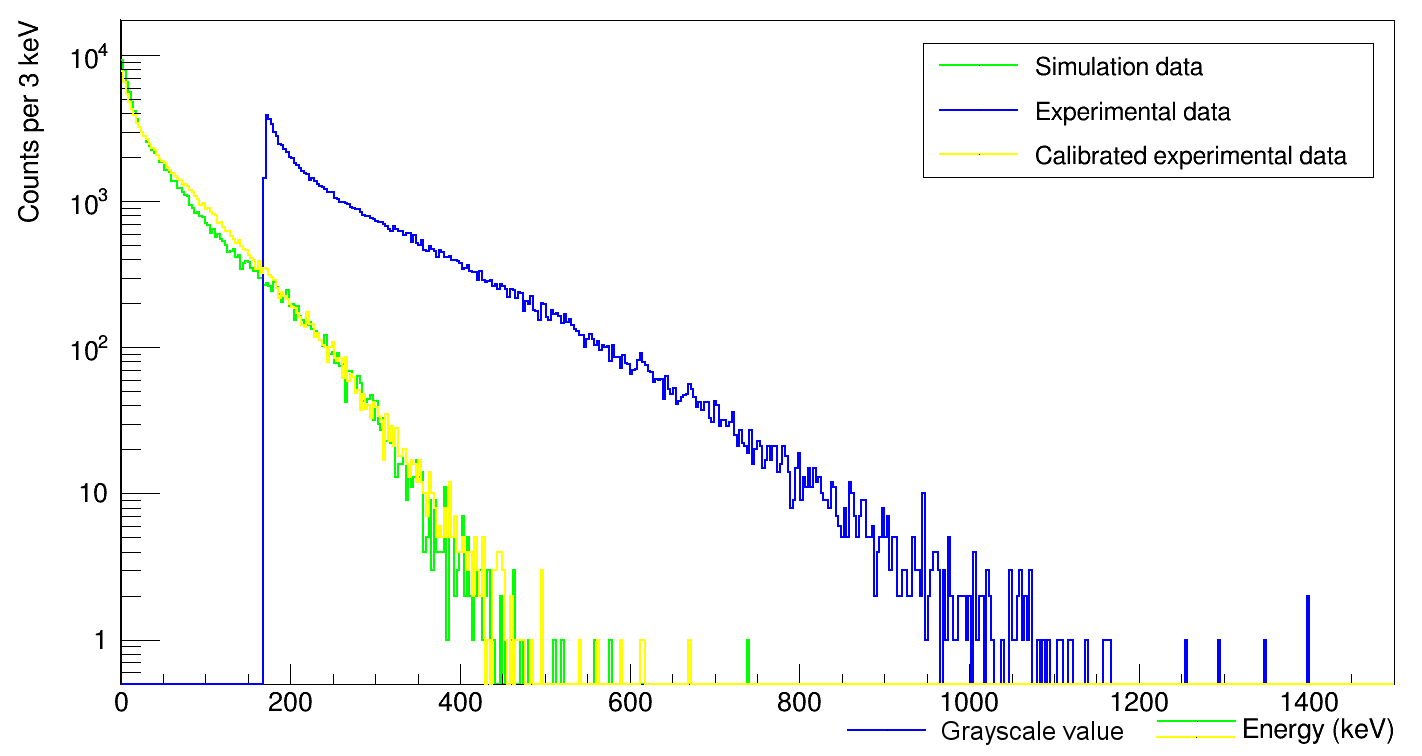
\includegraphics[width=0.8\linewidth,height=16cm]{Cs-calibrated.png}
\caption{Data from a $^{137}$Cs beta source, calibrated with a $\chi^2/$ndf of 7.2.}
\label{fig:cs}
\end{figure}

The data most commonly used comes from $^{14}$C, $^{90}$Sr, and $^{137}$Cs. Data from the simulation is used to characterize the system. A consistent calibration for all different sources has not yet been successful and needs to be explored.

\end{block}

%----------------------------------------------------------------------------------------

\end{column} % End of column 2.2

\end{columns} % End of the split of column 2

\end{column} % End of the second column

\begin{column}{\sepwid}\end{column} % Empty spacer column

\begin{column}{\onecolwid} % The third column

%----------------------------------------------------------------------------------------
%	CONCLUSION
%----------------------------------------------------------------------------------------

\begin{block}{Conclusion}

SLIMER has shown its capability to detect different types of radioactive decay. Furthermore, the G\textsc{eant}4 simulation has proven to be a useful tool in understanding and refining the experiment. The work in progress to calibrate data and demonstrate high position resolution will further the development of SLIMER as a useful tool in microbial ecology.

\end{block}

\begin{figure}
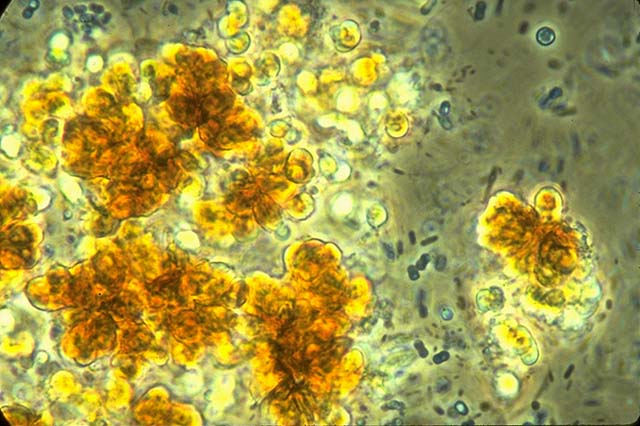
\includegraphics[width=0.8\linewidth]{alpinebiofilm.jpg}
\caption{A microscopic view of a biofilm of the type SLIMER eventually plans to analyze. Photo from [3].}
\label{fig:biofilm}
\end{figure}

%----------------------------------------------------------------------------------------
%	REFERENCES
%----------------------------------------------------------------------------------------

\begin{block}{References}

\nocite{*} % Insert publications even if they are not cited in the poster
\small{\bibliographystyle{unsrt}
\bibliography{sample}\vspace{0.75in}}

\end{block}

%----------------------------------------------------------------------------------------
%	CONTACT INFORMATION
%----------------------------------------------------------------------------------------

\begin{alertblock}{Contact Information}

\begin{itemize}
\item \href{mailto:egbuchanan42@students.tntech.edu}{\texttt{egbuchanan42@students.tntech.edu}}
\item \href{mailto:mkidd@tntech.edu}{\texttt{mkidd@tntech.edu}}
\item \href{mailto:elliotts@lanl.gov}{\texttt{elliotts@lanl.gov}}
\item \href{mailto:rielagek@lanl.gov}{\texttt{rielagek@lanl.gov}}
\end{itemize}

\end{alertblock}

%----------------------------------------------------------------------------------------

\end{column} % End of the third column

\end{columns} % End of all the columns in the poster

\end{frame} % End of the enclosing frame

\end{document}
